\subsubsection{O Círculo Trigonométrico}

A relação fundamental $\sen^2 \widehat B + \cos^2 \widehat B = 1$
sugere que os pontos do plano cartesiano $\paren{\cos \widehat B,
\sen \widehat B}$ pertencem a uma circunferência de raio 1, como
mostra a Imagem~\ref{fig:circulo-trigonometrico-b}.
%
\begin{figure}
\centering
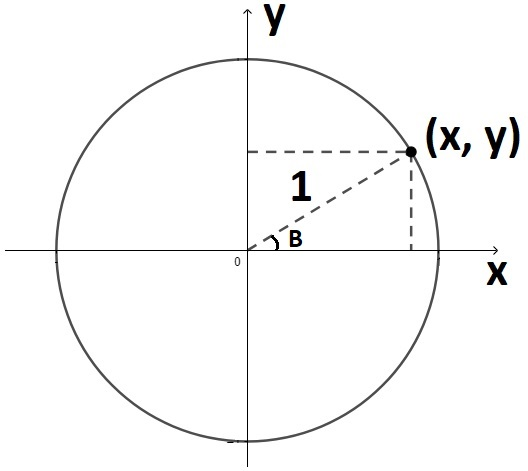
\includegraphics[scale=0.5]{\imgdirfromsection/circtrigB.jpg}
\caption{Pontos da forma $(\cos \widehat B, \sen \widehat B$ numa circunferência de raio 1.}
\label{fig:circulo-trigonometrico-b}
\end{figure}

Dessa forma, sendo $\widehat B$ o ângulo medido a partir do eixo
positivo de $x$ e tomando o sentido anti-horário como sentido
positivo, os pontos $(x, y)$ do círculo acima são tais que $x = \cos
\widehat B$ e $y = \sen \widehat B$.